\documentclass[a4paper]{article}

\usepackage{amsmath}
\usepackage{cleveref}
\usepackage{tikz}
\usetikzlibrary{automata, positioning, arrows}

\usepackage{graphicx}
\graphicspath{ {./static/} }

\tikzset{
->, % makes the edges directed
>=stealth, % makes the arrow heads bold
node distance=3cm, % specifies the minimum distance between two nodes. Change if necessary.
every state/.style={thick, fill=gray!10}, % sets the properties for each ’state’ node
initial text=$ $, % sets the text that appears on the start arrow
}

\begin{document}

\title{Backwards Compatible Automata}
\author{José Duarte \and Roland Kuhn}
\date{\today}
\maketitle

\section*{Theory-ish}

We will start by defining one of the simplest state machines — a light bulb.
Using the classical model, the light bulb automata can be defined as follows:

\begin{equation}
    (\Sigma, S, s_0, \delta, F) = (\{click\}, \{\text{Off}, \text{On}\}, \text{Off},S \times \Sigma \rightarrow S, \text{Off})
    \label{eq:fsm_long}
\end{equation}

However, for our purposes we do not need to care for the start nor final states,
for the sake of brevity we will remove them from our automata definitions going forward,
as well as the transition function (which is implicitly defined by stating that our state machines must be DFA).
Hence, we can express our light bulb as follows:

\begin{equation}
    (\Sigma, S) = (\{click\}, \{\text{Off}, \text{On}\})
    \label{eq:fsm_short}
\end{equation}

Which we can observe in \cref{fig:bulb_fsm}.
The bulb has two states — \emph{On} and \emph{Off} — both of which transition on the application of the symbol $\text{click}$.

\begin{figure}[ht]
    \centering
    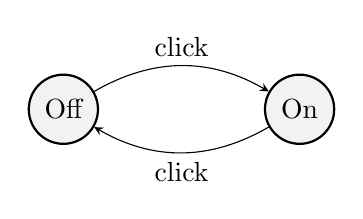
\begin{tikzpicture}
        \node[state] (Off) {Off};
        \node[state, right of=Off] (On) {On};


        \draw (Off) edge[bend left, above] node{click} (On);
        \draw (On) edge[bend left, below] node{click} (Off);
    \end{tikzpicture}
    \caption{Light bulb FSM}
    \label{fig:bulb_fsm}
\end{figure}

\subsection*{Let there be light}

Consider now that we are tasked with changing the state from carrying a boolean to a number,
describing the current light bulb intensity.
% Foreshadowing
Maybe in the future, the manufacturer wants the system to work with potentiometers.
To that end, we change the state machine definition from \cref{eq:fsm_short}
to the following (\cref{eq:fsm_intensity} and \cref{fig:bulb_fsm_intensity}):

\begin{equation}
    (\Sigma, S) = (\{click\}, \{0, 1\})
    \label{eq:fsm_intensity}
\end{equation}

\begin{figure}[ht]
    \centering
    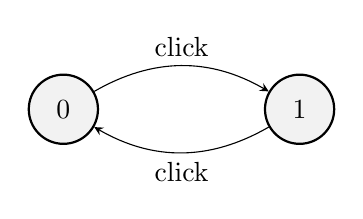
\begin{tikzpicture}
        \node[state] (0) {0};
        \node[state, right of=0] (1) {1};

        \draw (0) edge[bend left, above] node{click} (1);
        \draw (1) edge[bend left, below] node{click} (0);
    \end{tikzpicture}
    \caption{Light bulb FSM with Light intensity}
    \label{fig:bulb_fsm_intensity}
\end{figure}

% I'm dumping the swarm here out of nowhere, this of course, needs an introduction
At first sight, this is not a problem, in code we can just replace the old boolean for an integer,
this would be fine if every node of the swarm could be required to update, but that is not the case.
To cope with said problem, we need to map the old states to the new ones,
using Cambria \cite{Cambria2020} we can convert state information (see \cref{fig:bulb_fsm_state_cambria}).

\begin{figure}[ht]
    \centering
    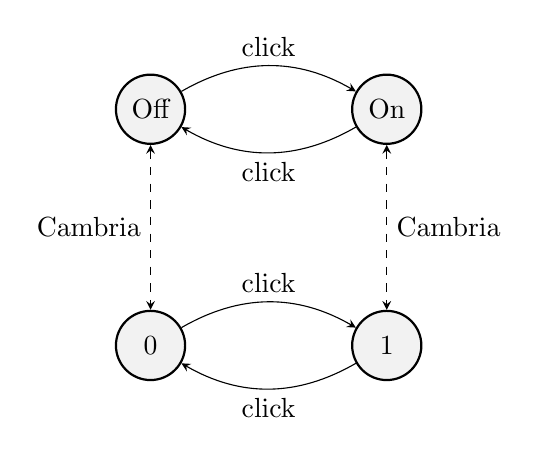
\begin{tikzpicture}
        % Named FSM
        \node[state] (Off) {Off};
        \node[state, right of=Off] (On) {On};

        \draw (Off) edge[bend left, above] node{click} (On);
        \draw (On) edge[bend left, below] node{click} (Off);

        % Intensity FSM
        \node[state, below of=Off] (0) {0};
        \node[state, below of=On] (1) {1};

        \draw (0) edge[bend left, above] node{click} (1);
        \draw (1) edge[bend left, below] node{click} (0);

        \draw (Off) edge[left, <->, dashed] node{Cambria} (0);
        \draw (On) edge[right, <->, dashed] node{Cambria} (1);
    \end{tikzpicture}
    \caption{Light bulb FSM with Cambria state mapping}
    \label{fig:bulb_fsm_state_cambria}
\end{figure}

Along with state conversion, we can extend Cambria to event labels (see \cref{fig:bulb_fsm_event_cambria}),
which is arguably an even better match since the labels (or payloads for more involved cases)
are what cross the network boundary.

\begin{figure}[ht]
    \centering
    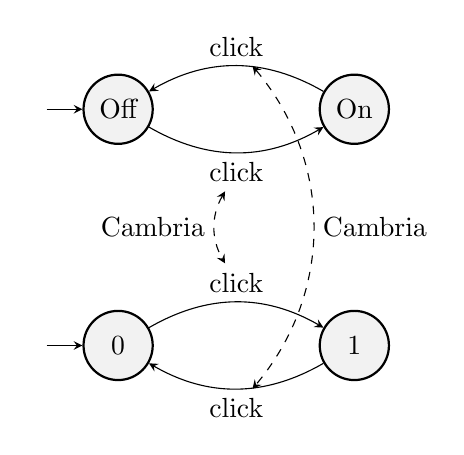
\begin{tikzpicture}
        % Named FSM
        \node[state, initial] (Off) {Off};
        \node[state, right of=Off] (On) {On};

        \draw (On) edge[bend right, above] node (v1-click-off) {click} (Off);
        \draw (Off) edge[bend right, below] node (v1-click-on) {click} (On);

        % Intensity FSM
        \node[state, initial, below of=Off] (0) {0};
        \node[state, below of=On] (1) {1};

        \draw (0) edge[bend left, above] node (v1'-click-on) {click} (1);
        \draw (1) edge[bend left, below] node (v1'-click-off) {click} (0);

        \draw (v1-click-on) edge[bend right, left, <->, dashed] node {Cambria} (v1'-click-on);
        \draw (v1-click-off) edge[bend left=40, right, <->, dashed] node {Cambria} (v1'-click-off);
    \end{tikzpicture}
    \caption{Light bulb FSM with Cambria event mapping}
    \label{fig:bulb_fsm_event_cambria}
\end{figure}

There is still an issue left to address: \emph{How does the old state machine know about new transformations?}
— to which the answer is simple — \emph{It does not know. It cannot know.}

If the old machine were able to get the new transformation,
it would mean that it could get the new state machine as well,
so we need to assume it cannot get the new Cambria transformation.

Thus, we are dealing with an asymmetric scenario where to keep the system running,
the most up-to-date system needs to pick up the slack from the older participants.
To do so, the up-to-date system can either pre-process all information going in and out
(as shown in \cref{fig:cambria_on_node_translation}) or require that all participants are
at least capable of running arbitrary Cambria transformations and exchange data with
the information of which transformations to apply along with the data
(as shown in \cref{fig:cambria_payload_with_translation}).

\begin{figure}
    \centering
    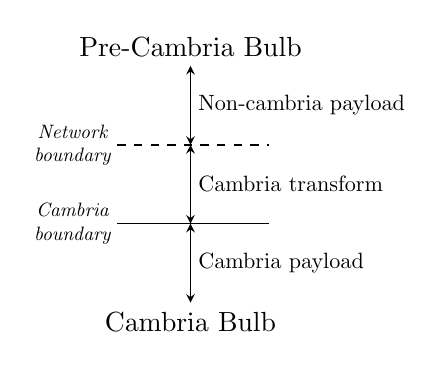
\begin{tikzpicture}
        \node (pre-cambria) at (0, 1.25) {Pre-Cambria Bulb} ;
        \node (cambria) at (0, -2.25) {Cambria Bulb};
        \node[align=center, scale=0.7, font=\itshape] (network) at (-1.5, 0) {Network\\boundary};
        \node[align=center, scale=0.7, font=\itshape] (cambria-b) at (-1.5, -1) {Cambria\\boundary};

        \draw[-, dashed, thick] (network) -- (1, 0);
        \draw[-] (cambria-b) -- (1, -1);

        \draw[<->] (pre-cambria) -- node[right, scale=0.8]{Non-cambria payload} (0, 0);
        \draw[<->] (0, 0) -- node[right, scale=0.8]{Cambria transform} (0, -1);
        \draw[<->] (cambria) -- node[right, scale=0.8]{Cambria payload} (0, -1);
    \end{tikzpicture}
    \caption{Asymmetric interaction between two bulbs, using Cambria to mediate data between them.}
    \label{fig:cambria_on_node_translation}
\end{figure}

\begin{figure}
    \centering
    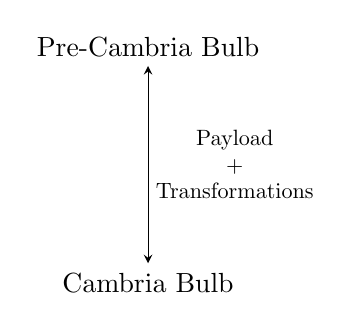
\begin{tikzpicture}
        \node (pre-cambria) {Pre-Cambria Bulb} ;
        \node[below of=pre-cambria] (cambria)  {Cambria Bulb};
        \draw[<->, align=center, right] (pre-cambria) -- node[scale=0.8]{Payload\\$+$\\Transformations} (cambria);
    \end{tikzpicture}
    \caption{Asymmetric interaction between two bulbs, using Cambria to mediate data between them.}
    \label{fig:cambria_payload_with_translation}
\end{figure}


\subsection*{Proper transforms now}

Once again, consider the light bulb using the intensity as states,
imagine that a new change was requested — instead of a toggle, we are now using
a button that can switch intensity from $0$, to $0.5$, to $1$ and back to $0$ (see \cref{eq:fsm_clicker}).

\begin{equation}
    (\Sigma, S) = (\{click\}, \{0, 0.5, 1\})
    \label{eq:fsm_clicker}
\end{equation}

\begin{figure}[ht]
    \centering
    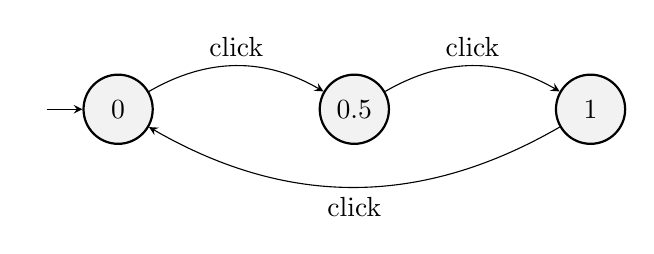
\begin{tikzpicture}
        \node[state, initial] (0) {0};
        \node[state, right of=0] (05) {0.5};
        \node[state, right of=05] (1) {1};

        \draw (0) edge[bend left, above] node{click} (05);
        \draw (05) edge[bend left, above] node{click} (1);
        \draw (1) edge[bend left, below] node{click} (0);
    \end{tikzpicture}
    \caption{Light bulb with support for multiple intensities (as defined in \cref{eq:fsm_clicker}).}
    \label{fig:bulb_fsm_multi_intensity}
\end{figure}

Usually, we would first design the new state machine (see \cref{fig:bulb_fsm_multi_intensity})
code it and ship it off as an update to the existing software, replacing the previous state machine.
However, as previously discussed, our system cannot afford the luxury of keeping everyone's version in sync,
so, if we want to support the previous version participants,
we need to keep processing their messages and moving the state machine along.

To support the previous state machine, we start by merging both state machines,
in a more formal way, we can define $merge(M_1, M_2)$
(where $M_1$ and $M_2$ are automata as defined in \cref{eq:fsm_short}) as:

\begin{equation}
    merge(M_1, M_2) = (M_1.\Sigma \cup M_2.\Sigma, M_1.S \cup M_2.S)
    \label{eq:fsm_merge}
\end{equation}

\begin{figure}[ht]
    \centering
    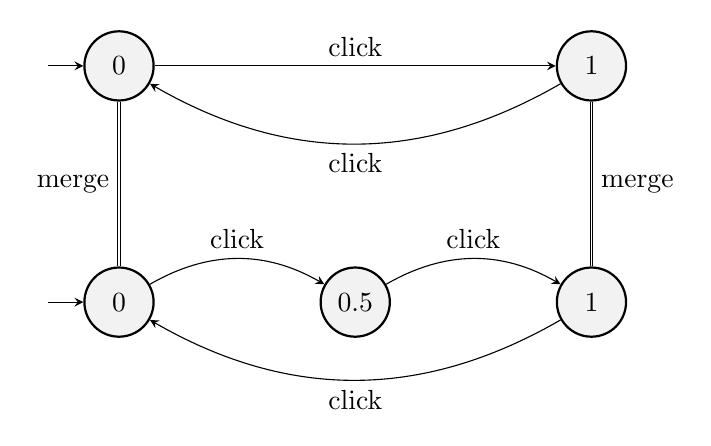
\begin{tikzpicture}
        \node[state, initial] (0) {0};
        \node[state, right of=0] (05) {0.5};
        \node[state, right of=05] (1) {1};

        \draw (0) edge[bend left, above] node{click} (05);
        \draw (05) edge[bend left, above] node{click} (1);
        \draw (1) edge[bend left, below] node{click} (0);

        \node[state, initial, above of=0] (0') {0};
        \node[state, above of=1] (1') {1};

        \draw (0') edge[above] node{click} (1');
        \draw (1') edge[bend left, below] node{click} (0');

        \draw (0) edge[double, -, left] node{merge} (0');
        \draw (1) edge[double, -, right] node{merge} (1');
    \end{tikzpicture}
    \caption{
        Visual approximation of $merge(M_1, M_2)$,
        where $M_1$ is the state machine from \cref{fig:bulb_fsm} and
        $M_2$ is the state machine from \cref{fig:bulb_fsm_intensity}.}
    \label{fig:bulb_fsm_merge}
\end{figure}



\begin{equation}
    \begin{split}
        merge(M_1, M_2) & = (\{click\} \cup \{click\}, \{0, 1\} \cup \{0, 0.5, 1\}) \\
        & = (\{click\}, \{0, 0.5, 1\})
    \end{split}
    \label{eq:merge_m1_m2}
\end{equation}

\Cref{eq:merge_m1_m2} shows the result of merging the state machines from
\cref{eq:fsm_intensity,eq:fsm_clicker}, however, while the result is accurate according to
the rules we established so far, it creates a problem that is not obvious when the resulting
state machine is represented in text.
If we display the result in a diagram (see \cref{fig:bulb_fsm_merge_nfa}) it becomes apparent —
the state machine is now non-deterministic (notice the two outgoing edges from state \emph{0} with the same \emph{click} label).

% I should probably add this transform as an appendix or something
We can to make it deterministic, which will result in a single state with a self loop.
This happens because our state machine's semantics are different from traditional
state machines (or acceptors), our state machine expresses behavior and acceptors
express a string matching mechanism. % This needs way better text and citations
Hence, we cannot use a traditional determinization algorithm and must rather, define our own approach.

The proposed solution is to label edges based on their version, thus removing collisions when merging.
By attributing versions to labels we are able to preserve the original states and keep the state machine deterministic
as shown in \cref{fig:bulb_fsm_merge_dfa}.
The versioning mechanism is left up to the state machine designer,
for the current work, we have opted to prefix a simple version (v1, v2, etc) to the label.

\begin{equation}
    \begin{split}
        merge(M_1, M_2) & {}= (\{v1.click\} \cup \{v2.click\}, \{0, 1\} \cup \{0, 0.5, 1\}) \\
        & {}= (\{v1.click, v2.click\}, \{0, 0.5, 1\})
    \end{split}
    \label{eq:fsm_merge_fixed}
\end{equation}


\begin{figure}[ht]
    \centering
    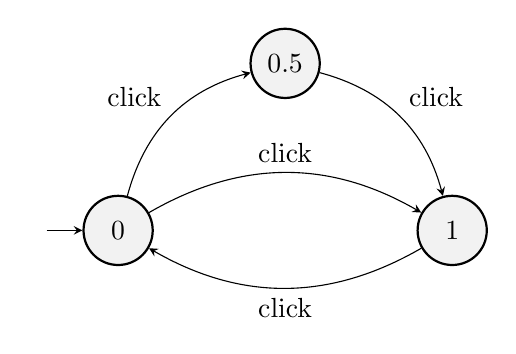
\begin{tikzpicture}
        \node[state, initial] (0) {0};
        \node[state, above right of=0] (05) {0.5};
        \node[state, below right of=05] (1) {1};

        \draw (0) edge[bend left, above left] node{click} (05);
        \draw (0) edge[bend left, above] node{click} (1);
        \draw (05) edge[bend left, above right] node{click} (1);
        \draw (1) edge[bend left, below] node{click} (0);
    \end{tikzpicture}
    \caption{$merge(M_1, M_2)$ results in an NFA (\cref{eq:fsm_merge}).}
    \label{fig:bulb_fsm_merge_nfa}
\end{figure}

\begin{figure}[ht]
    \centering
    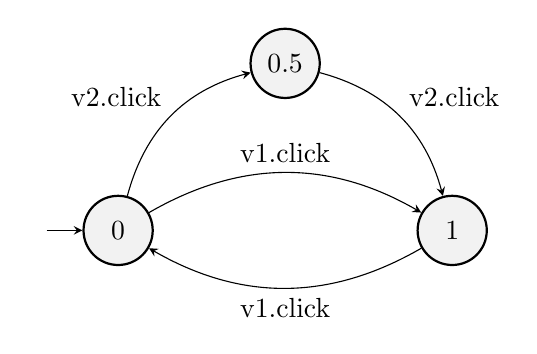
\begin{tikzpicture}
        \node[state, initial] (0) {0};
        \node[state, above right of=0] (05) {0.5};
        \node[state, below right of=05] (1) {1};

        \draw (0) edge[bend left, above left] node{v2.click} (05);
        \draw (0) edge[bend left, above] node{v1.click} (1);
        \draw (05) edge[bend left, above right] node{v2.click} (1);
        \draw (1) edge[bend left, below] node{v1.click} (0);
    \end{tikzpicture}
    \caption{$merge(M_1, M_2)$  with the new labels preserves the DFA (\cref{eq:fsm_merge_fixed}).}
    \label{fig:bulb_fsm_merge_dfa}
\end{figure}

Having solved the determinism issue, consider now a living room where the lights are controlled by
two distinct buttons, the first one is only able to send \emph{v1.click}s and the
second one is only able to send \emph{v2.click}s.
Consider the trace from \cref{eq:trace_1,eq:trace_2};
in \cref{eq:trace_1} someone toggled the lights to half intensity by using the second button,
followed by \cref{eq:trace_2} where someone clicked the button, but no action is taken.
Looking back to \cref{fig:bulb_fsm_merge_dfa}, we can see that state \emph{0.5} does not
have any way of handling \emph{v1.click}.
This is problematic because it means that one of the buttons is useless until the state machine
goes back to a state that supports it, breaking backwards compatibility.

\begin{subequations}
    \begin{align}
        \delta(0, v2.click)   & \rightarrow 0.5 \label{eq:trace_1} \\
        \delta(0.5, v1.click) & \rightarrow~? \label{eq:trace_2}
    \end{align}
\end{subequations}

To fix this, we require that each new version be complete regarding previous versions'
symbols, that is, each new version state must handle \emph{all} state labels from previous versions.

% Recursive definition here, but M_n really is all previous versions and the current one.
More formally, consider two state machines $M_n$ and $M_{n+1}$ (where $M_n$ represents all previous versions, or $M_n = M_1 \cup M_2 \cup \dots \cup M_n$),
we require that all new states have transitions accounting for all states of previous versions:
\begin{equation}
    \forall l \in M_n.\Sigma, s \in M_{n+1}.S, \exists s' \in (M_n.S \land M_{n+1}.S) : s \times l \rightarrow s'
\end{equation}

With that in mind, $M_2$ defined in \cref{eq:fsm_clicker} needs to be redefined (see \cref{eq:fsm_clicker_revisited});
resulting in the state machine displayed in \cref{fig:bulb_fsm_merge_dfa_upgraded}.

\begin{equation}
    (\Sigma, S) = (\{v1.click, v2.click\}, \{0, 0.5, 1\})
    \label{eq:fsm_clicker_revisited}
\end{equation}


\begin{figure}[ht]
    \centering
    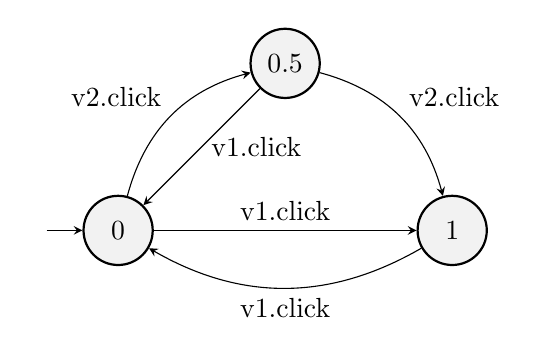
\begin{tikzpicture}
        \node[state, initial] (0) {0};
        \node[state, above right of=0] (05) {0.5};
        \node[state, below right of=05] (1) {1};

        \draw (0) edge[bend left, above left] node{v2.click} (05);
        \draw (05) edge[right] node{v1.click} (0);
        \draw (0) edge[above] node{v1.click} (1);
        \draw (05) edge[bend left, above right] node{v2.click} (1);
        \draw (1) edge[bend left, below] node{v1.click} (0);
    \end{tikzpicture}
    \caption{The result of $merge(M_1, M_{2}')$, where $M_{2}'$ is defined in \cref{eq:fsm_clicker_revisited}.}
    \label{fig:bulb_fsm_merge_dfa_upgraded}
\end{figure}

\section*{Forward compatibility}

So far, we have addressed backwards compatibility, that is, a state machine that is further ahead
is able to support messages from previous versions without conflicts. However, for the whole system to work,
old machines need to support messages from new versions without breaking.
The main challenge now lies in ensuring that while allowing state machines with different version to diverge
they still converge to the same state.

Consider now the state machines from \cref{fig:bulb_fsm_intensity,fig:bulb_fsm_merge_dfa},
if we run a trace composed of $[v2.click, v2.click]$, the state machines diverge, not being able to
converge on the previously existing state (as shown in \cref{tab:transition_breakage}).
Furthermore, if we consider the trace $[v2.click, v1.click]$ we can observe a similar issue (see \cref{tab:transition_breakage_2}),
the state machines are not able to converge due to a clear incompatibility in their transitions.

\begin{table}[ht]
    \centering
    \begin{tabular}{l|l|l|}
        \cline{2-3}
                                          & $V_1$ & $V_2$ \\ \hline
        \multicolumn{1}{|l|}{$\emptyset$} & 0     & 0     \\ \hline
        \multicolumn{1}{|l|}{v2.click}    & 0     & 0.5   \\ \hline
        \multicolumn{1}{|l|}{v2.click}    & 0     & 1     \\ \hline
    \end{tabular}
    \caption{We can see both state machines do not converge and thus generate a protocol breakage.}
    \label{tab:transition_breakage}
\end{table}

\begin{table}[ht]
    \centering
    \begin{tabular}{l|l|l|}
        \cline{2-3}
                                          & $V_1$ & $V_2$ \\ \hline
        \multicolumn{1}{|l|}{$\emptyset$} & 0     & 0     \\ \hline
        \multicolumn{1}{|l|}{v2.click}    & 0     & 0.5   \\ \hline
        \multicolumn{1}{|l|}{v1.click}    & 1     & 0     \\ \hline
    \end{tabular}
    \caption{We can see both state machines do not converge and thus generate a protocol breakage.}
    \label{tab:transition_breakage_2}
\end{table}

Fixing this requires replacing the $0.5$ state's outgoing edges with a single v1.click edge,
as shown in \cref{fig:bulb_fsm_converge}.
If we now revisit \cref{tab:transition_breakage,tab:transition_breakage_2},
the first table is now "incomplete" since it does not end in a state common to both versions,
thus, the event sequence needs to changed to $[v2.click, v1.click]$.
When running the new event sequence against our revisited version of the automata both
state machines converge to the same state, as shown in \cref{tab:transition_convergence}.

\begin{figure}[ht]
    \centering
    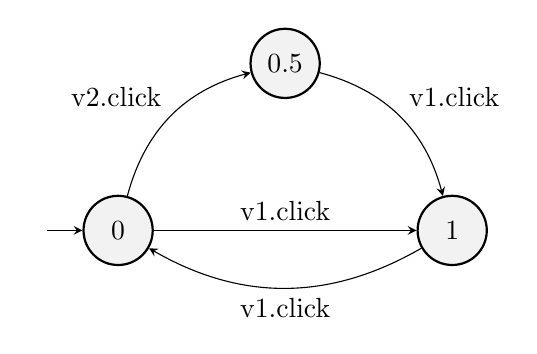
\begin{tikzpicture}
        \node[state, initial] (0) {0};
        \node[state, above right of=0] (05) {0.5};
        \node[state, below right of=05] (1) {1};

        \draw (0) edge[bend left, above left] node{v2.click} (05);
        \draw (0) edge[above] node{v1.click} (1);
        \draw (05) edge[bend left, above right] node{v1.click} (1);
        \draw (1) edge[bend left, below] node{v1.click} (0);
    \end{tikzpicture}
    \caption{Reworked automata with convergence in mind.}
    \label{fig:bulb_fsm_converge}
\end{figure}

\begin{table}[ht]
    \centering
    \begin{tabular}{l|l|l|}
        \cline{2-3}
                                          & $V_1$ & $V_2$ \\ \hline
        \multicolumn{1}{|l|}{$\emptyset$} & 0     & 0     \\ \hline
        \multicolumn{1}{|l|}{v2.click}    & 0     & 0.5   \\ \hline
        \multicolumn{1}{|l|}{v1.click}    & 1     & 1     \\ \hline
    \end{tabular}
    \caption{After changing the versioned automata, they now both converge to the same common state.}
    \label{tab:transition_convergence}
\end{table}

This works because both semantically and practically, the original path is kept intact,
to the older version, there's still a path to the state 1, to the new version, there are paths to
states 0.5 and 1, with the former converging to 1.

Extending the state machine can be done in two ways, extending an existing path (just as we have been doing),
or creating a completely new path. One might be tempted to generalize the approach we used previously,
but that approach quickly fails when creating a completely new path as demonstrated in \cref{tab:transition_extension_breakage,fig:fsm_extension_breakage}.

\begin{figure}[ht]
    \centering
    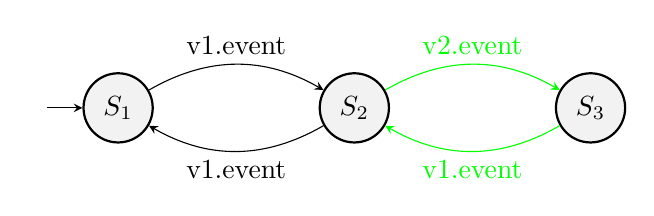
\begin{tikzpicture}
        \node[state, initial] (S1) {$S_1$};
        \node[state, right of=S1] (S2) {$S_2$};
        \node[state, right of=S2] (S3) {$S_3$};

        \draw (S1) edge[bend left, above] node{v1.event} (S2);
        \draw (S2) edge[bend left, below] node{v1.event} (S1);
        \draw (S2) edge[green, bend left, above] node{v2.event} (S3);
        \draw (S3) edge[green, bend left, below] node{v1.event} (S2);
    \end{tikzpicture}
    \caption{The green edges are the most recent additions to the state machine, extending $S_2$.}
    \label{fig:fsm_extension_breakage}
\end{figure}

\begin{table}[ht]
    \centering
    \begin{tabular}{l|l|l|}
        \cline{2-3}
                                          & $V_1$ & $V_2$ \\ \hline
        \multicolumn{1}{|l|}{$\emptyset$} & $S_1$ & $S_1$ \\ \hline
        \multicolumn{1}{|l|}{v1.event}    & $S_2$ & $S_2$ \\ \hline
        \multicolumn{1}{|l|}{v2.event}    & $S_2$ & $S_3$ \\ \hline
        \multicolumn{1}{|l|}{v1.event}    & $S_1$ & $S_2$ \\ \hline
    \end{tabular}
    \caption{Once more, the state machines do not converge.}
    \label{tab:transition_extension_breakage}
\end{table}

Hence, when adding completely new paths, the same rules do not apply and the proper fix here is to
use $v2.event$ instead of $v1.event$.

\begin{figure}[ht]
    \centering
    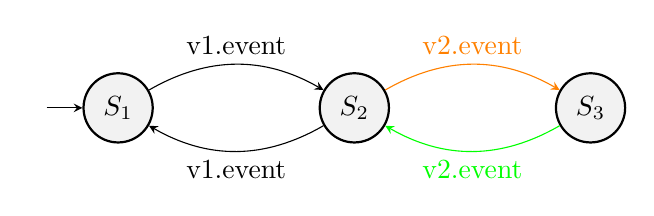
\begin{tikzpicture}
        \node[state, initial] (S1) {$S_1$};
        \node[state, right of=S1] (S2) {$S_2$};
        \node[state, right of=S2] (S3) {$S_3$};

        \draw (S1) edge[bend left, above] node{v1.event} (S2);
        \draw (S2) edge[bend left, below] node{v1.event} (S1);
        \draw (S2) edge[orange, bend left, above] node{v2.event} (S3);
        \draw (S3) edge[green, bend left, below] node{v2.event} (S2);
    \end{tikzpicture}
    \caption{The colored edges are the most recent additions to the state machine, extending $S_2$.}
    \label{fig:fsm_extension_breakage_fixed}
\end{figure}

\begin{table}[ht]
    \centering
    \begin{tabular}{l|l|l|}
        \cline{2-3}
                                          & $V_1$ & $V_2$ \\ \hline
        \multicolumn{1}{|l|}{$\emptyset$} & $S_1$ & $S_1$ \\ \hline
        \multicolumn{1}{|l|}{v1.event}    & $S_2$ & $S_2$ \\ \hline
        \multicolumn{1}{|l|}{v2.event}    & $S_2$ & $S_3$ \\ \hline
        \multicolumn{1}{|l|}{v2.event}    & $S_2$ & $S_2$ \\ \hline
    \end{tabular}
    \caption{The state machines now converge.}
    \label{tab:transition_extension_breakage_fixed}
\end{table}

\section*{Runtime-ish}

The state machine must be executed in some type of runtime, which is required to support
a plugin mechanism, be it web assembly modules or OS DLLs.

The way new capabilities are added is additive, in the sense that the state machines are defined
for a single version and merged later (in a pseudo compilation phase that ensures that the current version
is compatible with the previous one and obeys the rules).

When creating a new version, the user shouldn't care to merge automatically, but should care about the
backwards compatible transitions.
The new state machine is described and an automatic checker should validate if both are
compatible, only then is can be "compiled".

Modules should either be additive, meaning that a new module carries only the delta of changes;
or they should be compiled with all previous versions and shipped in a single module.

% Figure this last detail out, it's really important
% The idea would be that the state is a struct carrying data and the new functions handle transitions
% if we have a bunch of free functions, our transitions are something like:
% transition_function(state, event) -> new state
% this way our modules can simply be added cumulatively
% we still need a dynamic dispatch mechanism to pick which function to run
% some kind of switch statement based on the event

% Implementing a PoC in Python is fairly easy, make a dict[(state, symbol), function] the delta function
% then adding new things is simple

\bibliographystyle{plain} % We choose the "plain" reference style
\bibliography{refs} % Entries are in the refs.bib file

\end{document}
